\rhead{DOCUMENTATION}


\chapter{Appui sur la documentation TRUST}
\lhead{Appui sur la documentation TRUST}
\rhead{DOCUMENTATION}
TrioCFD étant un Baltik de TRUST, toute la documentation de TRUST est applicable pour TrioCFD. Cette documentation de TRUST est disponible soit via la commande \texttt{trust -index} dans un terminal après avoir chargé l'environnement TRUST soit dans le répertoire \texttt{doc/TRUST} de TRUST. Cette documentation est composée de : \\
\begin{itemize}[label=$\Rightarrow$, font=\LARGE]
  \item \textbf{ La Documentation Générale}
  \begin{itemize}
    \item \textit{Release notes} : Elle détaille toutes les intégrations majeures ou les changements ayant un impact sur l'utilisation de TRUST entre deux livraisons de version. Elle est renseignée par le développeur à la fin de son développement/correctif. Pour chacun d'eux, une ligne est ajoutée précisant la date d'intégration dans la version en développement de TRUST, le code sur lequel le travail a eu lieu, la nature de la modification des sources est précisée (New feature, Major Change, Bug fixed,...) et termine par un bref descriptif du travail (figure \ref{figure:RN-TRUST}).\newline
    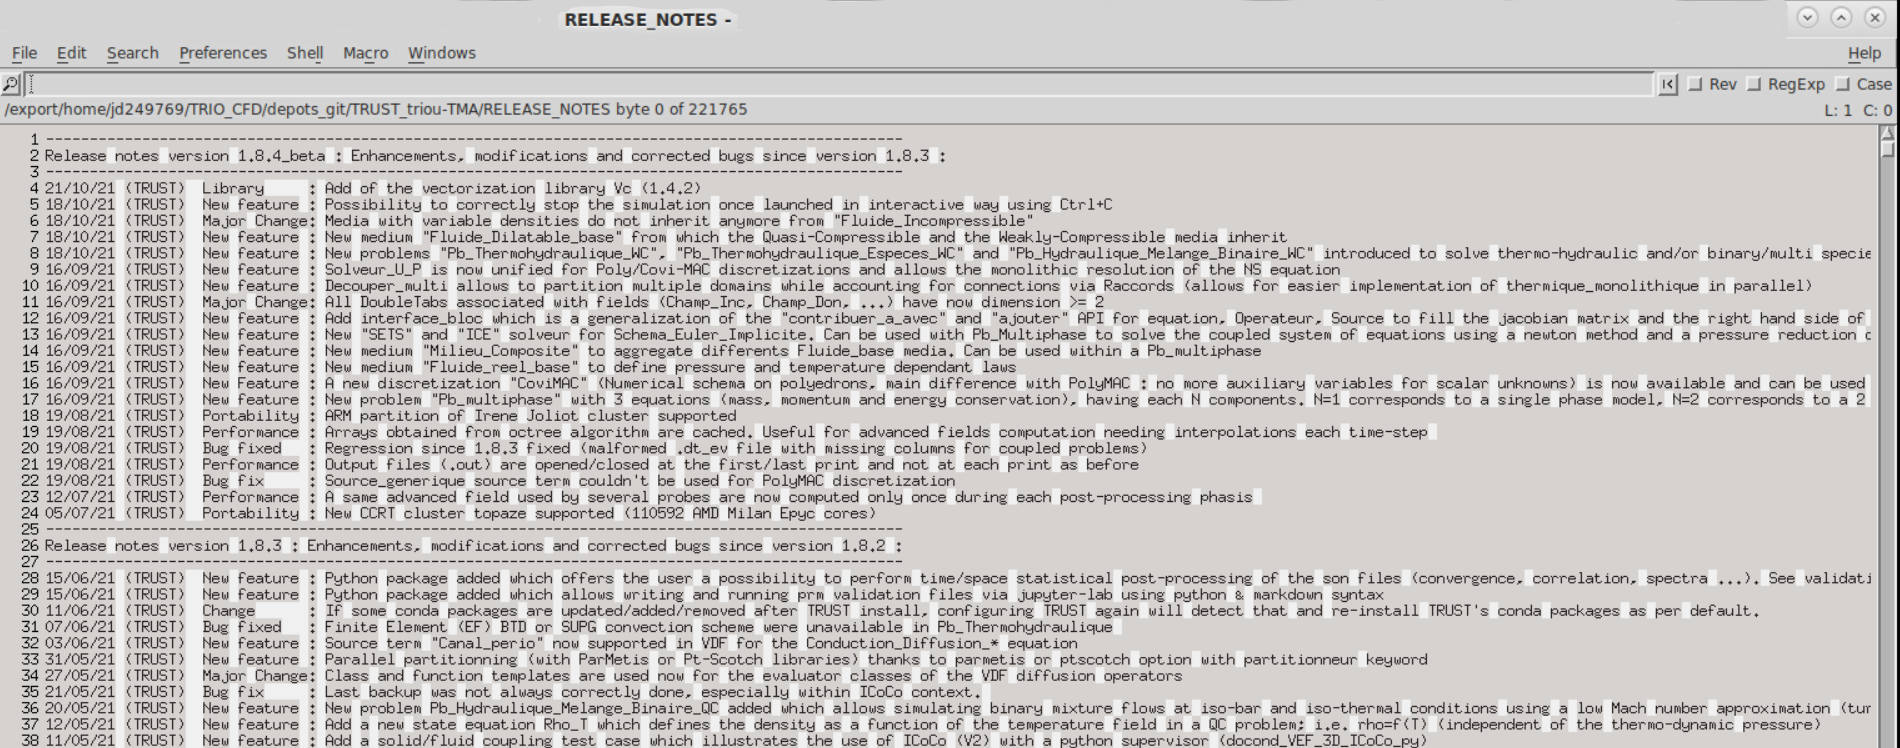
\includegraphics[width=14.5cm]{pictures/RN-TRUST.png}\vspace*{0.1cm}
   \captionof{figure}{\label{figure:RN-TRUST}Release notes de TRUST}
  \end{itemize}
  \begin{itemize}  
    \item \textit{Generic Guide} : Ce guide est le premier document à lire lorsque l'on commence à utiliser la plateforme TRUST. Il présente la plateforme TRUST de façon générale, décrit la méthodologie de lancement des cas-tests, la constitution générale d'un jeu de données, la méthodologie de post-traitement et de lancement d'un calcul en mode parallèle. 
    \item \textit{Reference Manual} : Il est généré automatiquement à partir des balises XDATA présentes dans le code et définies par le développeur. Ce manuel explicite tous les mots clés de TRUST et détaille la façon de les mettre en œuvre dans le jeu de données
    \item \textit{Description note} : Cette note, établie en 2007, présente les différents modèles et équations résolus par Trio\_U puisqu'elle a été émise avant la séparation TRUST/TrioCFD et n'a pas été mise à jour depuis. En ce qui concerne les informations de TrioCFD, celles-ci ne sont pas à prendre en compte dans cette documentation puisqu'une version à jour de ces aspects est présente dans la note spécifique à TrioCFD, nommée \texttt{Description des mod\`eles} (voir section \ref{subsec:modeles}).
    \item \textit{Best practices note} : Tout comme le document précédent, celui-ci, émis en 2013, concerne à la fois TRUST et TrioCFD puisqu'il s'agit d'un guide de bonnes pratiques pour la base de validation de Trio\_U. La partie concernant TrioCFD de cette note a été mise à jour avec la sortie de la documentation spécifique à TrioCFD à savoir le \texttt{Rapport de validation} (voir section \ref{subsec:validation}).
    \item \textit{Validation note} : Cette note émise en 2009 décrit l'organisation de la base de données des cas tests de validation de Trio\_U ainsi que la méthodologie mise en place pour leur automatisation. Comme la note précédente, les informations relevant de TrioCFD ont été mises à jour dans le \texttt{Rapport de validation} (voir section \ref{subsec:validation}).
  \end{itemize}
  \item \textbf{Ressources pour les utilisateurs}
  \begin{itemize}
    \item \textit{User tutorial} : ce tutoriel, à destination des utilisateurs de TRUST et TrioCFD, propose de nombreux exemples et exercices afin de prendre en main l'utilisation de la plateforme. Ce tutoriel est largement utilisé dans la formation utilisateur dispensée par l'équipe TMA.
    \item \textit{Test cases} : tableau récapitulatif des cas tests de référence de TRUST
    \item \textit{Keywords} : tableau de tous les mots clés de TRUST avec lien vers 1 ou plusieurs cas tests utilisant chacun d'eux.
    \item \textit{Memo scripts} : petit mémo des principaux scripts devant être connus par les utilisateurs de TRUST dans leurs prémices sur la plateforme.
  \end{itemize}
  \item \textbf{Ressources pour les développeurs}
  \begin{itemize}
    \item \textit{Developer tutoral} : ce tutoriel, à destination des développeurs de TRUST ou de tout Baltik sous base TRUST, propose de nombreux exemples et exercices afin de prendre en main le codage sur la plateforme. Ce tutoriel est largement utilisé dans la formation développeur dispensée par l'équipe TMA.
    \item \textit{ICoCo tutorial} : ce tutoriel explique la principe de couplage disponible sur la plateforme TRUST grâce à l'outil ICoCo (Interface for Code Coupling), comment le mettre en œuvre sur TRUST et TrioCFD via des exercices et des descriptions de méthodologie pas à pas.
    \item \textit{Other baltik tutorial} : il s'agit d'un document expliquant la création d'un Baltik sous base TRUST. Dans le cadre de TrioCFD, elle est également très utile pour créer des Baltiks ou des sous-Baltiks de TrioCFD, la méthodologie étant la même.
    \item \textit{C++ classes} : documentation DOxygen des classes de TRUST afin d'avoir une vision générale des classes de TRUST, des méthodes rattachées à celles-ci et une description des variables. Elle est générée automatiquement avec la commande \texttt{trust -gui} à partir des balises DOxygen présentes dans le code. Pour les parties de code non balisées, des scripts spécifiques ont été conçus afin qu'elles soient néanmoins prises en compte dans cette documentation indispensable aux développeurs.
    \item \textit{Test coverage} : tableau récapitulatif du nombre de lignes testées dans la partie \texttt{source} de TRUST mais également sur l'ensemble du projet TRUST.
    \item \textit{.prm syntax} : page html expliquant les différents éléments de syntaxe pour la création d'une fiche PRM (fiche de Validation). Si la majorité des mots clés sont applicables à TrioCFD, une nouvelle structure a été mise en place en 2020 dans TrioCFD et les nouveaux mots clés sont décrits dans le rapport de validation de TrioCFD qui sera présenté dans le chapitre suivant.
  \end{itemize}
\end{itemize} 
  
  
\chapter{\label{chapitre:doc-trio}Documentation spécifique à TrioCFD}
\lhead{Documentation spécifique à TrioCFD}
\rhead{DOCUMENTATION}
Outre cette documentation de TRUST, TrioCFD dispose de sa propre documentation en complément. Une grande partie de celle-ci a été mise en place récemment (à partir de 2019) afin de fournir d'avantage de supports à la communauté TrioCFD mais également d'accroître la qualité du code. Jusqu'alors les ressources humaines n'étaient pas suffisantes pour mener de front l'enrichissement des modèles et la mise en qualité. L'ensemble de ces documents sont gérés en gestion de configuration (sous GIT). Ils sont régulièrement enrichis et mis à jour au fur et à mesure des évolutions du code. En effet, leur mise à jour est une étape obligatoire dans tous les processus d'actions menées sur TrioCFD et ils sont relus, au même titre que le code à proprement parler, avant d'être intégrés dans la version. Mise à part la Release Notes qui est un simple document texte, ils sont tous en latex et disposent de leur propre script de génération. Les sources latex de ces documents sont accessibles dans le répertoire \texttt{/share/doc\_src} et disposent d'un répertoire spécifique chacun. Les fichiers PDF correspondants sont, quant à eux, disponibles dans le répertoire \texttt{/share/doc}. Tout comme TRUST, TrioCFD dispose d'une page Html facilitant l'accès à ces différents documents, qui peut être ouverte par la commande \texttt{triocfd -index} après avoir chargé l'environnement TrioCFD.
\subsection{Release Notes}
TrioCFD dispose de sa propre Release notes qui présente la même structure que celle de TRUST : date d'intégration dans le code - code concerné - nature du travail - bref descriptif. Elle présente l'ensemble des modifications/évolutions majeures faites dans le code depuis la version v1.4.0 (mi-2002), version dans laquelle, elle a été mise en place pour la première fois. Elle est organisée par livraison afin que l'utilisateur soit bien informé des changements d'une version à l'autre.\\
Elle est également mise à jour par le développeur lorsque ses travaux font apparaître de nouvelles fonctionnalités dans le code ou modifient le fonctionnement ou les résultats des fonctionnalités existantes. Elle est relue au moment de l'intégration de la branche d'un développement dans le code. Il est recommandé à l'utilisateur de la consulter avant l'utilisation de toute nouvelle version. Des renseignements supplémentaires sur chacun des points peuvent être obtenus auprès de l'équipe de TMA ou du Responsable de Code.
\subsection{TrioCFD Reference Manuel}
Tout comme le Manuel de Reference de TRUST, celui de TrioCFD est généré automatiquement à partir les balises XDATA présentes dans le code et définies par les développeurs pour chaque implémentation de nouveau mot clé. En effet, ce manuel répertorie l'ensemble des mots-clés de TrioCFD à disposition des utilisateurs pour la construction des jeux de données. Il précise la syntaxe exacte à employer pour chacun et décrit brièvement leur utilité.\\
Si ce document n'est pas extrêmement ergonomique et convivial, il présente néanmoins l'intérêt d'avoir les informations sur les mots-clés directement dans le code, ce qui facilite son évolution et sa maintenance. Des travaux sont actuellement en cours afin de mettre en place une documentation des mots-clé plus accessible et riche.
\subsection{Plan de d\'eveloppement TrioCFD 2020-2025}
Sorti en 2019 sous la forme d'une note technique CEA, il a été mis en gestion de configuration début 2021 afin de le mettre à disposition des utilisateurs mais également pour en assurer la sauvegarde.\\
Comme son nom l'indique, il répertorie les développements et les actions de Recherche et Développement prévus dans le code pour la période 2020-2025. Il décrit le programme technique à réaliser et les ressources associées. Il ne concerne que le code de CFD monophasique aux échelles RANS et LES. Les travaux envisagés sur le module de CFD diphasique moyenné, les baltiks FT et IJK font l'objet de documents séparés. Aucune date n'est spécialement définie en face de chaque action. La démarche consiste plutôt à choisir, chaque année, en fonction des sollicitations des utilisateurs et des ressources disponibles, certaines de ces actions et à les traiter. Des développements non définis dans ce document peuvent également être menés afin de répondre aux besoins exprimés par des projets ou des industriels après la rédaction de ce document. Il représente néanmoins la ligne directrice de l'évolution que l'équipe de développeurs CEA souhaite donner au code. D'autre part, il est également possible que certaines actions identifiées à l'époque perdent de leur pertinence au cours du temps et ne soient finalement pas traitées. Finalement, il est à prévoir que certaines actions de R\&D, qui sont longues à réaliser par nature, seront initiées durant cette période et
s'achèveront au-delà de ce terme.
\subsection{\label{subsec:modeles}Description des mod\`eles}
La première version de cette description des modèles est également une note CEA émise en 2019 qui a été mise en gestion de configuration début 2021, en même temps que le document précédent. Cette note décrit les principaux modèles physiques du code de TrioCFD.\\
Dans ce document, la présentation des modèles se concentre
sur la description des écoulements monophasiques, incompressibles, Newtoniens et turbulents. Sa deuxième section rappelle les équations de conservation de masse, quantité de mouvement et d'énergie sont rappelées. Sont également rappelées les définitions des tenseurs de contraintes, de déformation et de rotation qui reviendront dans tout le document. La section se termine par une description des matrices
de masse et de rigidité lorsque le problème de Stokes est discrétisé par la méthode des Volumes-Éléments Finis (VEF). La section suivante présente les différentes approches qui permettent de simuler la
turbulence en LES (Large Eddy Simulations) et en RANS (Reynolds Averaged Navier-Stokes). Pour les modèles RANS, plusieurs modèles de type $\kappa-\epsilon$ sont présentés : le $\kappa-\epsilon$ standard, le $\kappa-\epsilon$ réalisable, et le $\kappa-\epsilon$ bas Reynolds.  Depuis la première version de cette note, le document a été enrichi avec les modèles présents dans les Baltiks Phase\_Field, ALE et Sensitivity\_Analysis. Ce document ne fait, à l'heure actuelle, pas état de l'ensemble de modèles présents dans TrioCFD mais est régulièrement enrichi avec les modèles déjà existants dans TrioCFD et les nouveaux modèles régulièrement développés.
\subsection{\label{subsec:validation}Rapport de validation}
Le rapport de validation a été mis en place fin 2020 et rendu disponible pour la première fois à la livraison de la version v1.8.2. Dès sa création, il a immédiatement été mis en gestion de configuration car il s'agit d'un document évolutif qui fournit aux utilisateurs des exemples d'utilisation de TrioCFD sur les domaines physiques couverts par le code.\\
Il commence par décrire la nouvelle syntaxe des fiches de validation qui a été justement mise en place pour la création de ce document. En effet, jusqu'alors chaque fiche de validation avait sa structure propre définie par son auteur. L'idée a été de mettre en place une structure définie et identique pour toutes les fiches de validation afin de faciliter la lecture et la compréhension de ce rapport. Dans la première version de ce rapport, les fiches de validation couvraient les domaines suivant :\
\begin{itemize}
   \item les écoulements laminaires
   \item les écoulements laminaires avec échanges thermiques
   \item les écoulements turbulents
   \item les écoulements turbulents avec échanges thermiques
   \item les écoulements diphasiques avec le Baltik de Front-Tracking
\end{itemize}
Chaque domaine contient 3 fiches de validation dont les résultats numériques obtenus avec TrioCFD sont comparés soit à l'analytique, soit à des résultats expérimentaux, soit aux résultats numériques obtenus avec d'autres codes. L'entrée d'une fiche de validation dans le rapport de validation nécessite la réécriture de la fiche afin de la mettre au nouveau format. Certaines fiches de validation ne sont également pas suffisamment consistantes pour avoir leur place au sein de ce rapport. Ceci explique pourquoi l'intégralité des fiches de TrioCFD ne figure pas dans ce rapport de validation.
En 2021, trois fiches de validation sur le Baltik ALE, Baltik permettant la modélisation des interactions fluide-structure, y ont été intégrées. Ce rapport sera progressivement enrichi avec de nouvelles fiches dans les domaines existants mais également avec de nouveaux domaines non abordés jusqu'ici.
\subsection{Plan de Gestion de Configuration}
Le PGC ou Plan de Gestion de Configuration de TrioCFD (ce présent document) est le dernier à rejoindre les nouveaux documents mis à disposition des utilisateurs de TrioCFD. Il est disponible, pour la première fois fin 2021 à l'occasion de la sortie de la version v1.8.4. Il a également été immédiatement placé en gestion de configuration, car il s'agit aussi d'un document évolutif qui sera enrichi et mis à jour pour chaque évolution ou modification des pratiques ou des outils du code.

